\clearpage
\section*{Apêndice A: Rastreabilidade das evidências}
\addcontentsline{toc}{section}{Apêndice A: Rastreabilidade das evidências}

Os três arquivos, \texttt{aula2\_bpsk\_MATHEUS.grc},\ \texttt{aula2\_qpsk\_MATHEUS.grc}\ e\ \texttt{aula2\_16qam\_MATHEUS.grc}, acompanham este relatório e compilam com o utilitário \texttt{grcc} do GNU Radio 3.10.9. Os valores da Tabela~\ref{tab:medido} foram calculados a partir de 5000 símbolos por modulação, obtidos pela execução dos mesmos blocos \textit{Random Source} e \textit{Chunks to Symbols}, com os mesmos parâmetros, ligados a um \textit{Vector Sink} em lugar dos instrumentos gráficos.

Quanto à origem das figuras, as capturas de fluxo são imagens reais do GNU Radio Companion abrindo cada arquivo \texttt{.grc}, acrescidas de um painel de texto com os parâmetros exatos, porque o aplicativo trunca a \textit{Symbol Table} dentro do bloco. As constelações e as saídas temporais da Seção~\ref{sec:res} foram redesenhadas com a biblioteca \textit{matplotlib} a partir dos dados capturados, de modo a incluir título, eixos, legendas e a identificação dos níveis. Para que não restem dúvidas sobre o comportamento dos instrumentos originais, o Apêndice B traz capturas reais das janelas dos \textit{QT GUI Sinks}.

Os \textit{scripts} que geram os arquivos \texttt{.grc}, executam a captura e produzem as figuras estão na pasta \texttt{scripts} do projeto, o que permite reproduzir todos os resultados. Ressalva-se que o GNU Radio Companion rotula o bloco \textit{Throttle} como \textit{old} (captura da Figura~\ref{fig:bpsk-fluxo}) e que o \texttt{grcc} emite um aviso de descontinuação, mas o bloco permanece funcional para o propósito desta atividade, que é limitar a taxa de amostras em \SI{32000}{} por segundo.

\section*{Apêndice B: Capturas reais dos QT GUI Sinks}
\addcontentsline{toc}{section}{Apêndice B: Capturas reais dos QT GUI Sinks}

As Figuras~\ref{fig:qt-bpsk} a~\ref{fig:qt-16qam} mostram as janelas dos instrumentos do próprio GNU Radio durante a execução dos três fluxogramas. Nelas, os rótulos de eixo são os padrões do aplicativo (\textit{In-phase}, \textit{Quadrature} e \textit{Time}), e o \textit{Time Sink} liga as amostras por segmentos de reta, o que difere dos degraus das figuras redesenhadas. A sequência aleatória dessa execução é independente da usada nos arquivos \texttt{.csv}.

\begin{figure}[H]\centering
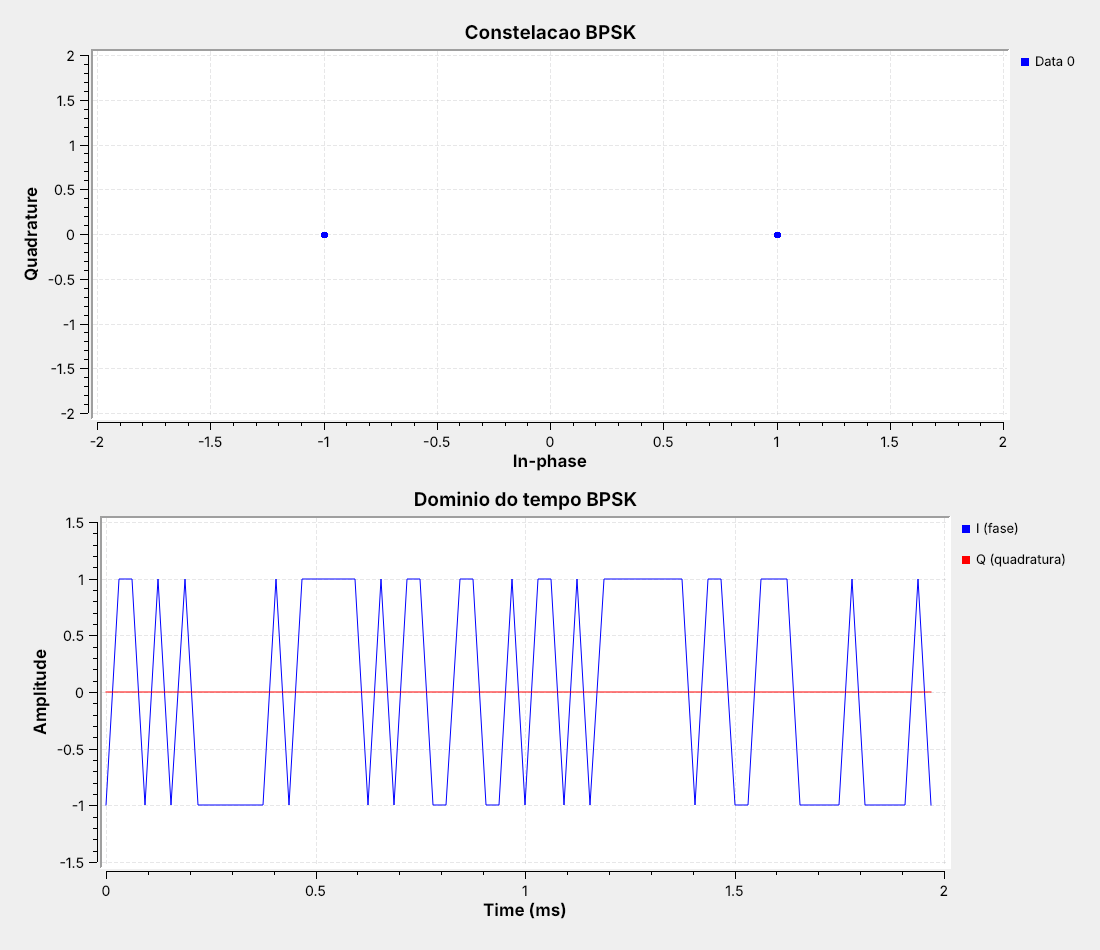
\includegraphics[width=0.78\linewidth]{figuras/extra_bpsk_qtgui_real.png}
\caption{Janela real dos instrumentos na BPSK}\label{fig:qt-bpsk}
\fonte{captura de tela da execução do fluxograma \texttt{aula2\_bpsk\_MATHEUS.grc}.}
\end{figure}
\begin{figure}[H]\centering
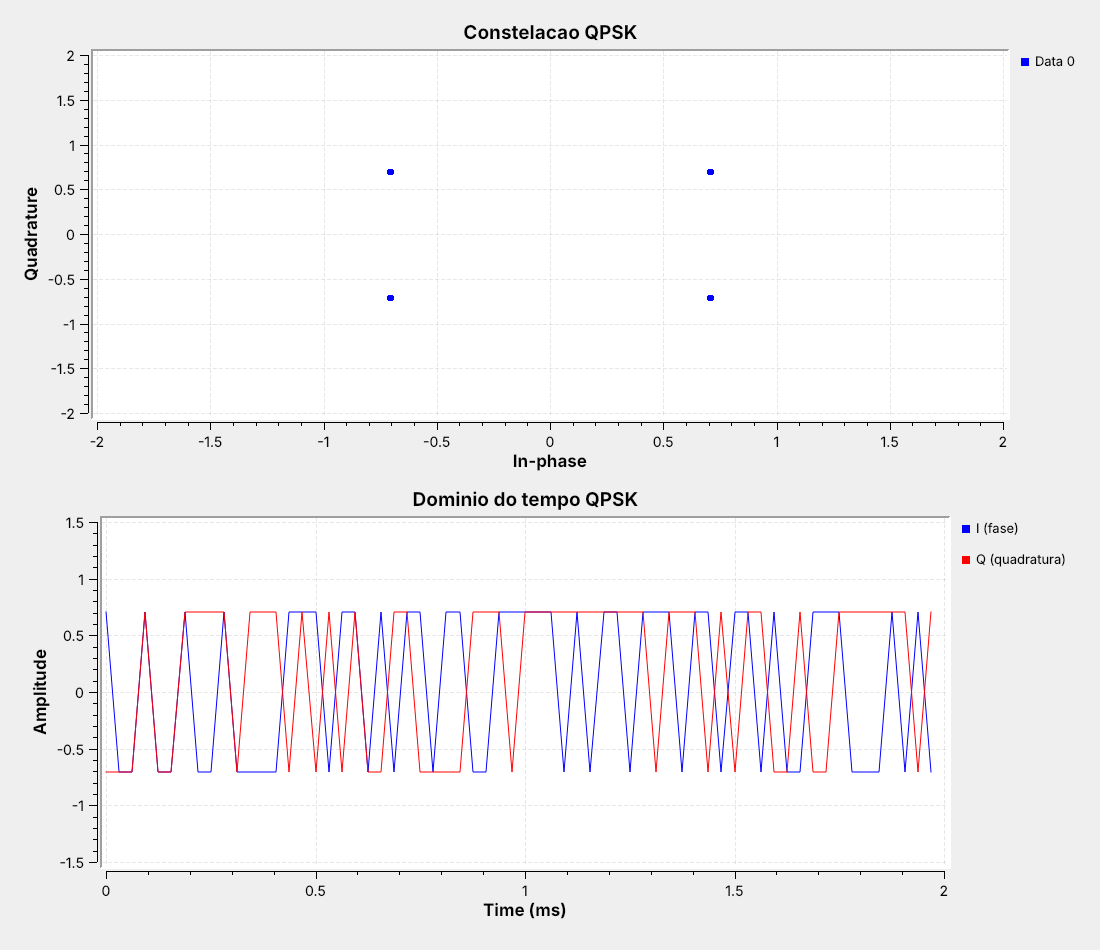
\includegraphics[width=0.78\linewidth]{figuras/extra_qpsk_qtgui_real.png}
\caption{Janela real dos instrumentos na QPSK}\label{fig:qt-qpsk}
\fonte{captura de tela da execução do fluxograma \texttt{aula2\_qpsk\_MATHEUS.grc}.}
\end{figure}
\begin{figure}[H]\centering
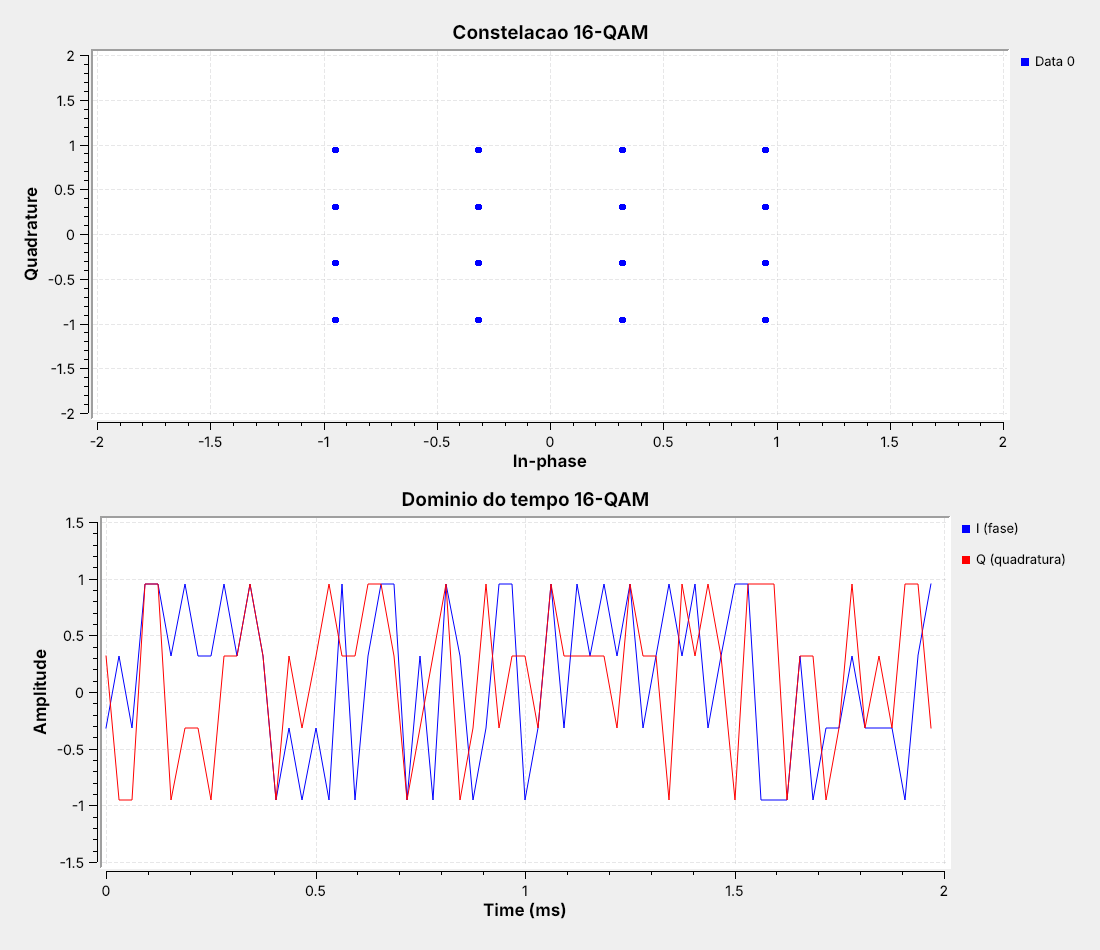
\includegraphics[width=0.78\linewidth]{figuras/extra_16qam_qtgui_real.png}
\caption{Janela real dos instrumentos na 16-QAM}\label{fig:qt-16qam}
\fonte{captura de tela da execução do fluxograma \texttt{aula2\_16qam\_MATHEUS.grc}.}
\end{figure}
